\documentclass[12pt,hyperref,]{ctexart}
\usepackage{lmodern}
\usepackage{amssymb,amsmath}
\usepackage{ifxetex,ifluatex}
\usepackage{fixltx2e} % provides \textsubscript
\ifnum 0\ifxetex 1\fi\ifluatex 1\fi=0 % if pdftex
  \usepackage[T1]{fontenc}
  \usepackage[utf8]{inputenc}
\else % if luatex or xelatex
  \ifxetex
    \usepackage{xltxtra,xunicode}
  \else
    \usepackage{fontspec}
  \fi
  \defaultfontfeatures{Mapping=tex-text,Scale=MatchLowercase}
  \newcommand{\euro}{€}
\fi
% use upquote if available, for straight quotes in verbatim environments
\IfFileExists{upquote.sty}{\usepackage{upquote}}{}
% use microtype if available
\IfFileExists{microtype.sty}{%
\usepackage{microtype}
\UseMicrotypeSet[protrusion]{basicmath} % disable protrusion for tt fonts
}{}
\usepackage[tmargin=2.5cm, bmargin=2.5cm, lmargin=3cm, rmargin=3cm]{geometry}
\ifxetex
  \usepackage[setpagesize=false, % page size defined by xetex
              unicode=false, % unicode breaks when used with xetex
              xetex]{hyperref}
\else
  \usepackage[unicode=true]{hyperref}
\fi
\usepackage[usenames,dvipsnames]{color}
\hypersetup{breaklinks=true,
            bookmarks=true,
            pdfauthor={},
            pdftitle={Handwriting Recognition Application Report},
            colorlinks=true,
            citecolor=blue,
            urlcolor=blue,
            linkcolor=magenta,
            pdfborder={0 0 0}}
\urlstyle{same}  % don't use monospace font for urls
\setlength{\emergencystretch}{3em}  % prevent overfull lines
\providecommand{\tightlist}{%
  \setlength{\itemsep}{0pt}\setlength{\parskip}{0pt}}
\setcounter{secnumdepth}{5}

\title{Handwriting Recognition Application Report}
\author{Xu Chen (徐晨)}
\date{August 24, 2019}
\usepackage{fontspec, xunicode, xltxtra}
\usepackage{xeCJK,ctex}
\usepackage{bm,xcolor}
\usepackage{fancyhdr}
\usepackage{url}
\usepackage{float}
\usepackage{graphicx}
\usepackage{pythonhighlight}
\usepackage{listings}
\lstset{ language=bash, basicstyle=\ttfamily }
\pagestyle{fancy}
\fancyhead[L]{Handwriting Recognition Application Report}
\renewcommand{\baselinestretch}{1.5}
\renewcommand{\headrule}{{\color{red}\hrule width\headwidth height\headrulewidth \vskip-\headrulewidth}}
\renewcommand{\footrule}{{\color{black}\vskip-\footruleskip\vskip-\footrulewidth \hrule width\headwidth height\footrulewidth\vskip\footruleskip}}
\renewcommand{\headrulewidth}{0.8pt}
\renewcommand{\footrulewidth}{0.6pt}
\renewcommand\contentsname{\bfseries CONTENT}
\renewcommand\tablename{table}
\renewcommand\figurename{figure}
\usepackage[sf,raggedright]{titlesec}
\usepackage{titletoc}
\titleformat{\section}{\bfseries\large\color{blue}}{\bfseries\thesection}{0.5em}{}
\titlespacing{\section}{0pt}{3.5ex plus .1ex minus .2ex}{1.5\wordsep}
\hypersetup{colorlinks=true, breaklinks=true, linkcolor=blue}

% Redefines (sub)paragraphs to behave more like sections
\ifx\paragraph\undefined\else
\let\oldparagraph\paragraph
\renewcommand{\paragraph}[1]{\oldparagraph{#1}\mbox{}}
\fi
\ifx\subparagraph\undefined\else
\let\oldsubparagraph\subparagraph
\renewcommand{\subparagraph}[1]{\oldsubparagraph{#1}\mbox{}}
\fi

\begin{document}
\maketitle

{
\setcounter{tocdepth}{2}
\tableofcontents
}
\newpage

\noindent\textbf{ACKNOWLEDGEMENT}:

Many people have offered me valuable help in my project, including my
mentor and my friends.

First, I would like to give my sincere gratitude to my mentor, Zhang
Fan, who taught me a lot of knowledge I have never learnt from my
college. He introduced some applications and methods which are
frequently used in big data analysis including Docker, Cassandra,
Tensorflow, etc. Without his support, I will have no access to those
powerful tools, and may not manage to build this app.

Then, I will thank my friends Zhang Yunneng and Qiao Dan. As experienced
programmers, they gave me tons of precious advice in programming with
their patience (Indeed, most of my questions are quite silly and easy to
find a solution on the internet).

\newpage

\noindent\textbf{ABSTRACTS}:

Handwriting recognition is the ability of a machine to receive and
interpret handwritten input. It involves different fields of subjects
including Computer Science, Statistics. The application of handwritting
recognition can be simutanously versatile, it is found widely used in
industries, banks, web service. The main task of this app is to receive
a handwritten picture with a number ranged from 0 to 9 on it and return
the prediction of the digit on the picture. We chose softmax regression
as our recognition model, and made it into a web app with flask and
python, users can post the picture via RESTful api, and store the data
in cassandra database. Finally we built a docker image of all the stuff
we talked, in order to ensure all users can run the app no matter what
operating system they are using.

\vspace{1.5cm} \textbf{Keywords:}

Image processing, Handwriting recognition, Softmax regression, Docker
container.

\newpage

\section{Introduction}\label{introduction}

\subsection{Object of the Projecst}\label{object-of-the-projecst}

The main task of this app is to receive a handwritten picture with a
number ranged from 0 to 9 and return the prediction of the digit on the
picture.

\subsection{Dataset}\label{dataset}

We use the MNIST database(\url{http://yann.lecun.com/exdb/mnist/}) as
our training dataset. The MNIST database of handwritten digits has a
training set of 60,000 examples, and a test set of 10,000 examples.

\begin{table}[H]
\caption{Summary of MNIST dataset}
\begin{center}
\begin{tabular}{|p{6cm}|p{8cm}|}
\hline
train-images-idx3-ubyte.gz & training set images (9912422 bytes) \\ \hline
train-labels-idx1-ubyte.gz &  training set labels (28881 bytes)\\ \hline
t10k-images-idx3-ubyte.gz &  test set images (1648877 bytes) \\ \hline
t10k-labels-idx1-ubyte.gz &   test set labels (4542 bytes)\\
\hline
\end{tabular}
\end{center}
\end{table}

Both training and testing dataset are dataframe with column number of
784 (28*28). It indicates that each row of the dataframe represents a
28-by-28 pixel image reshaped to a 1-by-784 vector.

\begin{figure}[H]
\centering
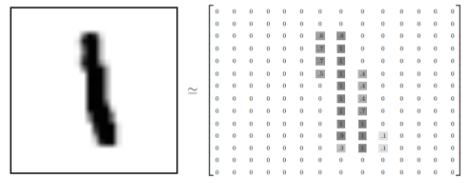
\includegraphics[width=5in]{pre.png}
\label{demo}
\end{figure}

\subsection{Softmax regression}\label{softmax-regression}

Softmax regression (or multinomial logistic regression) is a
generalization of logistic regression to the case where we want to
handle multiple classes.

In the softmax regression setting, we are interested in multi-class
classification (as opposed to only binary classification), and so the
label y can take on K different values, rather than only two. Thus, in
our training set \(\{(x^{(1)},y^{(1)}),…,(x^{(m)},y^{(m)})\}\)

Given a test input x, we want our hypothesis to estimate the probability
that \(P(y=k|x)\) for each value of \(k=1,…,K\) . I.e., we want to
estimate the probability of the class label taking on each of the K
different possible values. Thus, our hypothesis will output a
K-dimensional vector (whose elements sum to 1) giving us our K estimated
probabilities.

Our cost function will be:\\
\[J(\theta) = -\frac{1}{m}[\Sigma_{i=1}^m\Sigma_{j=1}{k}I_{y^{(i)=j}}
                            log\frac{e^{\theta^T_j}x^{(i)}}{\Sigma_{l=1}^k e^{\theta^T_l}x^{(i)}}]\]

we can apply an iterative optimization algorithm to find an approximate
solution.

\newpage

\section{Pre-Process}\label{pre-process}

In this section, we want to convert a image to the vector compatible
with the data structure in our model, that is to say we want to convert
any kind of images to a 1-by-784 vector. We use the following code to
meet the requirement.

Here comes the code for the pre-process of images.

\begin{python}
import tensorflow as tf
import numpy as np
from PIL import Image

def pre_pic(picName):
    img = Image.open(picName)
    reIm = img.resize((28, 28), Image.ANTIALIAS)
    
    #Change to grayscale
    im_arr = np.array(reIm.convert('L'))
    
    #threshold,reduce the noise
    threshold = 50
    for i in range(28):
        for j in range(28):
            im_arr[i][j] = 255 - im_arr[i][j]
            if(im_arr[i][j] < threshold):
                im_arr[i][j] = 0
            else: pass
    nm_arr = im_arr.reshape([1,784])
    
    #reshape
    nm_arr = nm_arr.astype(np.float32)
    img_ready = np.multiply(nm_arr, 1.0/255.0)

    return img_ready
\end{python}

\newpage

The Image() function is from module `pillow', we can change the scale of
the picture, and convert it to an 28-by-28 array, then reshape it to a
vector compatible with our model . For example, A denotes the vector
converted from the picture we post, we can \(AW+b\) which W and b are
the weight and bias matrix we defined as we mentioned in the previous
section. The answer of \(AW+b\) returns a vector, and if we do a
logistic transform on it, we can get the probility of each prediction.
The index of column which the maximum occurs is the predictions of that
picture. In the next section, i will show how \(W\) and \(b\) are
calculated.

\newpage

\section{Modelling}\label{modelling}

In the previous section, we can get the A matrix if the user post an
image. All we need to do is to get the \(W\) and \(b\) which can be
determined from the training dataset. We can define a loss function:
\(H_{y'}(y)=-\Sigma_i y_i'log(y_i)\) which is the cross-entropy
function. y is our predicted probability distribution, y' is the actual
distribution Then we use the gradient descent algorithm to minimize the
cross-entropy.\\
The code of this process can be found on github
\url{https://github.com/tensorflow/tensorflow/blob/r1.4/tensorflow/examples/tutorials/mnist/mnist_softmax.py}

The accuracy of the testing set is about 91\%, and we can say the model
is pretty efficient, taking the time of modelling into consideration(the
training is quite fast, it cost less than 1 min).

When the training is done, we can simply save the model in our hard
disk, and every time we want to use the model, just import the model we
trained in order to save time.

We add this code to mnist\_soft to save the model.

\begin{python}
  saver = tf.compat.v1.train.Saver()
  sess.run(accuracy, feed_dict={x: mnist.test.images,
                                      y_: mnist.test.labels})
  saver.save(sess,"Model/model.ckpt")
\end{python}

Now, if a user posts a new image, we can get the prediction of that
through the previous work.

\newpage

\section{Implement}\label{implement}

\subsection{Flask}\label{flask}

We can put the model in our flask app, then users can post images via
RESTful api.\\
Here is a fraction of code:

\begin{python}
import datetime
import os
from flask import Flask,request
from werkzeug.utils import secure_filename

app = Flask(__name__)

@app.route('/mnist',methods = ["GET","POST"])
def mnist():
    req_time = datetime.datetime.now()

    if request.method == "POST":
        f= request.files['file']
        upload_filename = secure_filename(f.filename)
        save_filename = str(req_time).rsplit('.',1)[0]+''+upload_filename
        save_filepath = os.path.join(app.root_path,'uploads',save_filename)
        f.save(save_filepath)
            
        img = pre_pic(save_filepath)
        pred = str(getPred(img)[0])
        return("%s%s%s%s%s%s%s%s%s" % ("Filepath: ",save_filepath,'\n',"Filename: ",save_filename,'\n',"Prediction: ",pred,"\n"))
        
if __name__ == '__main__':
    app.run(host='0.0.0.0',port=80)
\end{python}

This function is quite simple, when a user post an image, we rename the
file with the current timestamp and original filename, and save the
image to 'uploads'folder in the working directory,

We can post picuture using `curl' command with our terminal, for
example:

\begin{figure}[H]
\centering
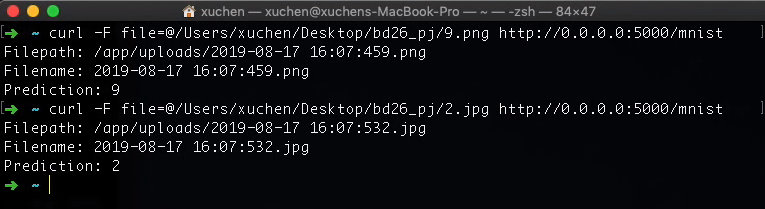
\includegraphics[width=6in]{curl.png}
\caption{post pictures using 'curl' command}
\end{figure}

\subsection{Cassandra}\label{cassandra}

Our initial idea is to build a remote database to store filename,
filepath, time and prediction. Therefore, instead of pulling a docker
image, we built a local cassandra database and wanted to make the
database into a remote database so we can view all the commit and the
status of each one. However, we didn't find an approach to visit the
database with WAN(Wide Area Network).

In our app,

\begin{python}
from cassandra.cluster import Cluster

clusterList=['192.168.0.102','127.0.0.1']
cluster=Cluster(clusterList)
session=cluster.connect("bd26_pj")
session.execute("INSERT INTO mnist(filename,path,time,prediction) VALUES
            (%s,%s,%s,%s)",[save_filename,save_filepath,req_time,pred])
\end{python}

192.168.0.102 is the ip address of my computer, we changed some
configuration in `cassandra.yaml' to broadcast, and consequently any
machine in the LAN can get access to the database.

\subsection{Docker}\label{docker}

Our app relies on python 3.7 and several modules including tensorflow,
flask, pillow. Therefore we build a docker image which ensure the app
can run on any kind of os which with docker installed. Just run the
following command in terminal, and we build all our codes into a docker
image.

\begin{figure}[H]
\centering
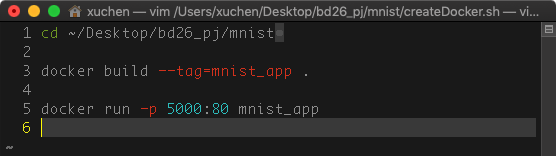
\includegraphics[width=6in]{docker.png}
\label{create docker image}
\end{figure}

\section{Testing and Results}\label{testing-and-results}

There are two pictures as my own testing data:

\begin{figure}[H]
\begin{minipage}[t]{0.5\linewidth}
\centering

\includegraphics[width=2.2in]{2.jpg}
\caption{2.jpg}
\label{fig:side:a}
\end{minipage}%
\begin{minipage}[t]{0.5\linewidth}
\centering

\includegraphics[width=2.2in]{9.png}
\caption{9.png}
\label{fig:side:b}
\end{minipage}
\end{figure}

The first one is made by myself with iPad, the second is downloaded from
internet. They both can be correctly recognized by our app, and here
comes the data we inserted into cassandra database:

\begin{figure}[H]
\centering
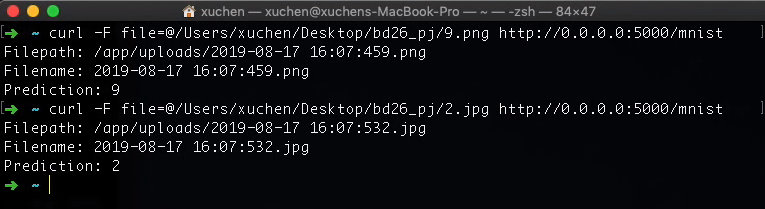
\includegraphics[width=6in]{curl.png}
\end{figure}

It appears that the accuracy is quite good. However i have encountered
several misclassification error:

\begin{figure}[H]
\centering
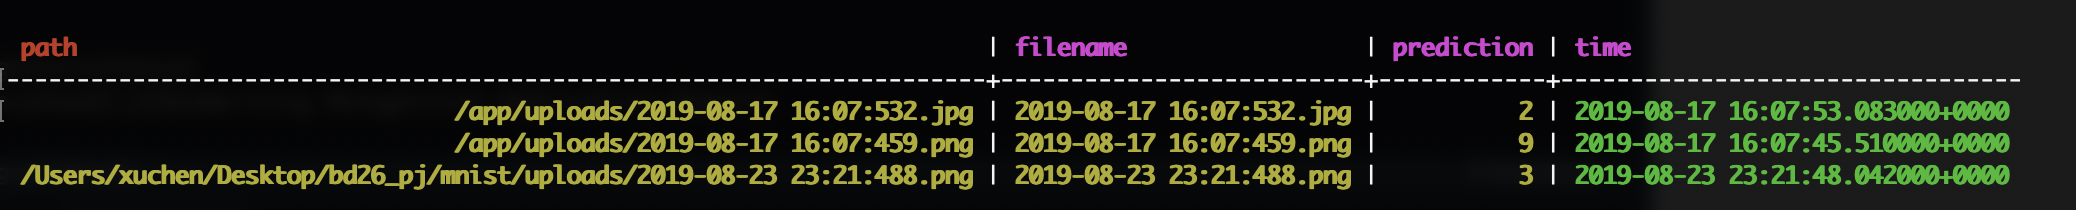
\includegraphics[width=5in]{cass.png}
\end{figure}

\begin{table}[H]
\caption{data inserted}
\begin{center}
\begin{tabular}{|p{4cm}|p{3.5cm}|p{1.8cm}|p{4cm}|}
\hline
path & filename & prediction & time \\ \hline
/app/uploads/2019-08-17 16:07:532.jpg & 2019-08-17 16:07:532.jpg & 2 & 2019-08-17 16:07:53.083000+0000\\
/app/uploads/2019-08-17 16:07:459.png & 2019-08-17 16:07:459.png & 9 & 2019-08-17 16:07:45.510000+0000\\
/Users/xuchen/Desktop /bd26pj/mnist/uploads /2019-08-23 23:21:488.png & 2019-08-23 23:21:488.png & 3 & 2019-08-23 23:21:48.042000+0000\\ 
\hline
\end{tabular}
\end{center}
\end{table}

The prediction is 3 instead of the true value 8. Though the picture is a
printed one, i don't know if it makes a differece.

\begin{figure}[H]
\centering

\includegraphics[width=2.2in]{8.png}
\caption{8.png}
\end{figure}

It's not easy for us to create our own testing dataset with a large
scale. However the built-in testing dataset shows that the accuracy is
above 90\% percent, and the training and testing are extract from a
larger dataset called NIST separated with stratified sampling. The two
dataset are independent, so we can believe that if add new testing
dataset, the misclassification rate will be no more that 10\%(if the
dataset is big enough).

\newpage

\section{Conclusions and remarks}\label{conclusions-and-remarks}

In our project, we made an app based on MNIST dataset and softmax
regression to do handwriting recognition. We receive the file users
posts via RESTful api, and write the data in canssandra database,
finally build all of them in a docker container. The prediction turns
out to be quite accurate. However, we didn't manage to use a remote
database with WAN, so currently, not every users can view all the commit
history of pictures posted and their prediction, and it need to be
improved in our next version(if it exists).

\section{Appendix}\label{appendix}

\subsection{code}\label{code}

\url{https://github.com/xckomorebi/mnist_app}

\end{document}
